\documentclass[]{article}
\usepackage{hyperref}
\usepackage{graphicx}
\usepackage{float}
\usepackage{cclicenses}
\usepackage{listings}

%opening
\title{FrameSquared}
\author{
	  Carbone, John\\
	\texttt{john@qlcorp.net}
	\and
	Erimez, Esra\\
	\texttt{eerimez@e24x7inc.com}
}

\begin{document}

\maketitle
\begin{tabular}{|p{.9\textwidth}|}
	\hline
	\begin{center}
		This work is licensed under a Creative Commons Attribution-ShareAlike 4.0 International License.
	\end{center}
\begin{center}
	\url{https://creativecommons.org/licenses/by-sa/4.0/}
\end{center}
	\begin{center}
		\includegraphics[scale=0.40]{cc-by-sa.png}
	\end{center}\\
	\hline
\end{tabular}

\begin{abstract}
FrameSquared performs database schema version control and scaffold generation for Postgres databases and the Treefrog C++ MVC framework using YAML to 
\end{abstract}


\section{Overview}
The rise of iterative and incremental software development methodologies has been transformative. Continuous integration\cite{ci}, deployment and delivery\cite{cd,cidd} has met the challenge of regular changes in requirements. Unpredictable and changing requirements\cite{bea} have been factored into the development process to enable software architectures to evolve gracefully.

Iterative and incremental methodologies have been successfully applied to database schema revision control and migration\cite{rd}. Refactoring database schema effects the database and related queries but also has repercussions to external systems that access the database programmatically, these include models and controllers. 

The nature of MVC frameworks lends itself to the use of boilerplate code. Some MVC frameworks create scaffolding using templates to generate boilerplate code. Scaffolding was made populate by Ruby-on-Rails. Most scaffold generators focus primarily on create, retrieve, update and delete (CRUD) operations using HTML\cite{scaffold,vsscaffold} and do not generally support single page applications\cite{spa} and associated messaging protocols such as SOAP or REST.

FrameSquared is tool that can generate code to be used as final source files and/or migrations based on serial numbers and up/down direction and can execute programs. FrameSquared uses the notion of "serial" numbers and "direction" to determine whether a migration "action" should be executed.


\section{Required Libraries}
FrameSquared utilizes the Inja\cite{inja} template engine which in turn uses the nlohmann JSON library\cite{nlohmann}. FrameSquared also makes heavy use to the nlohmann JSON library. FrameSquared also uses the jbeder YAML\cite{jbeder} library.



\begin{lstlisting}
Put your code here.
\end{lstlisting}



\begin{figure}[H]
	\centering
	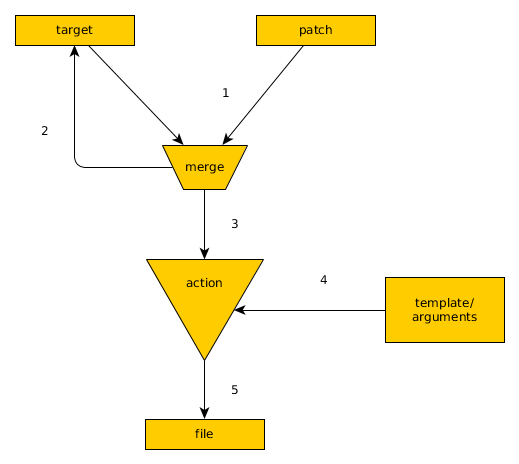
\includegraphics[scale=0.45]{fs2_merge.png}
	\caption{Merge Overview}
\end{figure}

\begin{thebibliography}{9}
\bibitem{ci}
Paul M. Duvall, Steve Matyas, Paul Duvall, Andrew Glover
\textit{Continuous Integration: Improving Software Quality and Reducing Risk}
Addison-Wesley, 2007

\bibitem{cd}
Jez Humble and David Farley
\textit{Continuous Delivery: Reliable Software Releases through Build, Test, and Deployment Automation}
Addison-Wesley, August 2010

\bibitem{cidd}
Sten Pitet
\textit{Continuous integration vs. continuous delivery vs. continuous deployment}
\url{https://www.atlassian.com/continuous-delivery/principles/continuous-integration-vs-delivery-vs-deployment}
Atlassian, Retrieved January 1st, 2019

\bibitem{bea}
Neal Ford, Rebecca Parsons, Patrick Kua
\textit{Building Evolutionary Architectures: Support Constant Change}
O'Reilly Media Inc, October 8, 2017

\bibitem{rd}
Scott J Ambler and Pramod J. Sadalage
\textit{Refactoring Databases: Evolutionary Database Design}
Addison-Wesley Professional, March 13, 2006

\bibitem{scaffold}
\textit{Scaffoling (programming)}
\url{https://en.wikipedia.org/wiki/Scaffold_(programming)}
Wikipedia, Retrieved January 1st, 2019

\bibitem{vsscaffold}
Nick Harrison
\textit{Using Scaffolding to Create MVC Applications with Visual Studio}
\url{https://www.red-gate.com/simple-talk/dotnet/asp-net/using-scaffolding-to-create-mvc-applications-with-visual-studio/}
www.red-gate.com, 14 December 2015

\bibitem{spa}
Paul Sherman
\textit{How Single-Page Applications Work:Getting to know the browser behaviors and APIs responsible for powering more and more web pages}
\url{https://medium.com/@pshrmn/demystifying-single-page-applications-3068d0555d46}
mediun.com, 11 April 2018

\bibitem{inja}
Inja
\textit{A Template Engine for Modern C++}
\url{https://github.com/pantor/inja}
GitHub

\bibitem{nlohmann}
JSON for Modern C++
\textit{A Template Engine for Modern C++}
\url{https://github.com/nlohmann/json/}
GitHub

\bibitem{jbeder}
YAML
\textit{A YAML parser and emitter in C++ }
\url{https://github.com/jbeder/yaml-cpp}
GitHub

\end{thebibliography}


\end{document}
